\documentclass[a4paper,11pt]{report}

\usepackage{lscape}
\usepackage{multirow,array}
\usepackage{booktabs}
\usepackage{newunicodechar}
\usepackage{xspace}
\usepackage[T1,OT1]{fontenc}
\usepackage{newtxtext,newtxmath}
\usepackage[top=1in, bottom=1in, left=1in, right=1in]{geometry}
\usepackage{amsmath}
\usepackage{amssymb}
\usepackage{listings}
\usepackage{graphicx}
\usepackage{blindtext}
\usepackage{enumitem}
\usepackage{mathtools}
\usepackage{color}
\usepackage[colorlinks=false,hidelinks]{hyperref}
\usepackage{needspace}
\usepackage{pdfpages}
\usepackage{easy-todo}
\usepackage{lipsum}
\usepackage{natbib}
\usepackage{tabularx}
\usepackage{algorithm}
\usepackage[noend]{algpseudocode}
\usepackage{multicol}
\usepackage{titlesec}
\usepackage{etoolbox}

%--- custom ---

\newcommand{\lang}[1]{\emph{#1}}
\newcommand{\er}{\textsuperscript{er} }
\newcommand{\e}{\textsuperscript{e} }
\newcommand{\ra}[1]{\renewcommand{\arraystretch}{#1}}

\makeatletter
\def\BState{\State\hskip-\ALG@thistlm}
\makeatother

\newcommand{\bin}{\in\{0,1\}}
\newcommand{\real}{\in \mathbb{R}^+}

\definecolor{codegreen}{rgb}{0,0.6,0}
\definecolor{codegray}{rgb}{0.5,0.5,0.5}
\definecolor{codepurple}{rgb}{0.58,0,0.82}
\definecolor{backcolour}{rgb}{0.95,0.95,0.92}
\lstdefinestyle{mystyle}{
    backgroundcolor=\color{backcolour},   
    commentstyle=\color{codegreen},
    keywordstyle=\color{magenta},
    numberstyle=\tiny\color{codegray},
    stringstyle=\color{codepurple},
    basicstyle=\footnotesize,
    breakatwhitespace=false,         
    breaklines=true,                 
    captionpos=b,                    
    keepspaces=true,                 
    numbers=left,                    
    numbersep=5pt,                  
    showspaces=false,                
    showstringspaces=false,
    showtabs=false,                  
    tabsize=2
}
\lstset{style=mystyle}

\DeclareMathOperator{\xor}{XOR}

% --- sectionning ---
\makeatletter
\renewcommand\@chapapp{Partie}

\newcommand\chapterwithsubtitle[2]{
  \chapter[#1: {\itshape#2}]{#1\\[2ex]\Large\itshape#2}
}

\def\@makechapterhead#1{%
  \vspace*{30\p@}%
  {\parindent \z@ \raggedright \normalfont
    \ifnum \c@secnumdepth >\m@ne
        \LARGE\bfseries\thechapter\quad
        %\vskip 20\p@
    \fi
    \interlinepenalty\@M
    \huge \bfseries #1
    %\vskip 40\p@
  }}
\makeatother
\setcounter{tocdepth}{2}

\titleformat{\chapter}
  {\normalfont\LARGE\bfseries}{\thechapter}{1em}{}
\titlespacing*{\chapter}{0pt}{3.5ex plus 1ex minus .2ex}{2.3ex plus .2ex}
\patchcmd{\chapter}{\if@openright\cleardoublepage\else\clearpage\fi}{}{}{}


\renewcommand\bibname{Références}
\renewcommand{\refname}{Références}
\makeatletter
\renewcommand\@biblabel[1]{#1.  }
\makeatother

% --- meta data ---
\title{Projet INFO-F-524}
\author{
	Antoine Passemiers \\
	Cédric Simar
}

% --- spec chars ---
\newunicodechar{’}{'}


\begin{document}

\renewcommand\bibname{References}
\renewcommand{\refname}{References}
\makeatletter
\renewcommand\@biblabel[1]{#1.  }
\makeatother

\begin{titlepage}
	\centering
	{\scshape\LARGE Université Libre de Bruxelles\par}
	\vfill
	{\LARGE\bfseries INFO-F-422 \\ Statistical foundations of Machine Learning \par
		\vspace{3ex}}
	{\itshape\Large Classifying Sample Covariance Matrices \\ using the geometry of Riemannian manifolds: \\\ \\ Application to Hand Motions Classification \par}
	\vfill
	\makeatletter
	{\large \@author\par}
	\vfill
	\@date\par
	\makeatother
\end{titlepage}

\tableofcontents

\setlength\parskip{0.5ex plus1ex minus.5ex}

\newpage



\chapter{Symmetric Definite Positive (SPD) matrices}

\section{Sample Covariance Matrices (SCMs) are Symmetric (Semi-)Definite Positive matrices}

A necessary preliminary for understanding the mechanics of Riemannian geometry is to convince ourselves that
SCMs are actually SPD matrices. Let $x_i = (x_{i1}, \ldots, x_{im})^T$ be a sequence of raw samples
located in a fixed time window, where $i \in \{1, \ldots, n\}$ is a time step, $k$ is the number of electrodes,
$m$ is the number of electrodes and $n$ is the number of samples.
Let $\mu_x$ be the vector of empirical means of those samples:

\begin{align}
  \mu_x & = \frac{1}{n} \sum\limits_{i=1}^{n} x_i
\end{align}

\noindent where the size of $\mu_x$ is equal to $m$ and element
$\mu_{x_i}$ is the empirical mean of samples from electrodes $i$.
Then the corresponding SCM $\Sigma$ is found by applying this formula on the raw samples:

\begin{align}
  \Sigma & = \frac{1}{n} \sum\limits_{i=1}^{n} (x_i - \mu_x) \ (x_i - \mu_x)^T
\end{align}

\noindent More specifically, the covariance $\Sigma_{ij}$ between electrodes $i$ and $j$
is given by $\frac{1}{n} \sum\limits_{k=1}^{n} (x_{ki} - \mu_{x_i}) \ (x_{kj} - \mu_{x_j})^T$.
For $\Sigma$ to be positive definite, the scalar $z^T \ \Sigma \ z$ must be strictly positive
for any non-zero vector $z \in \mathbb{R}^m$. Let's prove that this property holds:

\begin{align}
  z^T \Sigma z & = z^T \ \Big( \frac{1}{n} \sum\limits_{i=1}^{n} (x_i - \mu_x) \ (x_i - \mu_x)^T \Big) \ z \\
  & = \frac{1}{n} \sum\limits_{i=1}^{n} z^T \ (x_i - \mu_x) \ (x_i - \mu_x)^T \ z \\
  & = \frac{1}{n} \sum\limits_{i=1}^{n} \Big( (x_i - \mu_x)^T \ z \Big)^T \ \Big( (x_i - \mu_x)^T \ z \Big) \\
  & = \frac{1}{n} \sum\limits_{i=1}^{n} \Big( (x_i - \mu_x)^T \ z \Big)^2 \ge 0
\end{align}

Matrix $\Sigma$ is thus semi-positive definite. Also, one can reasonably assume that in most cases,
the SCM is such that all samples values are non-constant and that product $(x_i - \mu_x)^T \ z$
is different from zero for at least one time step. This allows us to confirm that $\Sigma$ is definite
positive. Also, it can be easily seen from the definition of $\Sigma$ that it is symmetric:

\begin{align}
  \Sigma^T & = \Big( \frac{1}{n} \sum\limits_{i=1}^{n} (x_i - \mu_x) \ (x_i - \mu_x)^T \Big)^T \\
  & = \frac{1}{n} \sum\limits_{i=1}^{n} \Big( (x_i - \mu_x) \ (x_i - \mu_x)^T \Big)^T \\
  & = \frac{1}{n} \sum\limits_{i=1}^{n} \Big( (x_i - \mu_x)^T \Big)^T \ \Big( (x_i - \mu_x) \Big)^T \\
  & = \frac{1}{n} \sum\limits_{i=1}^{n} (x_i - \mu_x) \ (x_i - \mu_x)^T \\
  & = \Sigma
\end{align}

\noindent SCMs are thus both symmetric and definite positive.

\section{SPD matrices lie on a convex cone}

Let $\mathcal{M}(n)$ be the set of $n \times n$ real matrices.
Also, let $\mathcal{P}(n)$ be the space of $n \times n$ symmetric positive-definite matrices defined as:
\begin{equation}
    \mathcal{P}(n) = \{ A \in \mathcal{M}(n), \ A^T = A, x^T A x > 0, x \in \mathbb{N} \backslash \{0\}
\end{equation}
$\mathcal{P}(n)$ is an open convex cone if, for all $P$ and $Q$ in $\mathcal{P}(n)$,
$P + tQ$ is in $\mathcal{P}(n) \ \forall t > 0$~\citep{doi:10.1137/S0895479803436937}.
It is indeed easy to see that, if $P$ and $Q$ are symmetric positive-definite, 
$P + tQ$ is also symmetric positive-definite \ $\forall t > 0$.

\section{Relation to EEG signal classification}

During a mental task, the EEG signal can be characterized by the covariant matrix estimated on a signal window of the length of the mental task. In this work, we hypothesize that the covariant matrix can be used reliably to describe the EEG signal associated with a specific mental task. Ultimately, the objective is to estimate a classification function $y_i = h(\Sigma_{i})$ that will map the covariant matrix $\Sigma_{i}$ to the associated hand movement class.


\chapter{Riemannian manifolds}

\section{Background}

Let's make a necessarily short description of what Riemannian manifolds are. They have a quite heavy
formalism, and rather simple ideas can become confusing if we stick to much to formulas. However, let's introduce them
properly by defining the notions of topological spaces, manifolds and Riemannian differential manifolds.

\subsection{Topological spaces}

Let's use the axiomatized definition of topological spaces from Hausdorff.
Let $X$ be a set and $N(x)$ a function that maps a point $x \in X$ to a set of neighbourhoods of $x$.
Then $X$ is a so-called topological space if the following axioms are satisfied:
\begin{itemize}
  \item The intersection of two neighbourhoods of $x$ belongs to $N(x)$.
  \item For any set in $N(x)$, $x$ belongs to it ($x$ is located in its own neighbourhoods).
  \item Any subset of $X$ that contains a neighbourhood of $x$, is itself a neighbourhood of $x$.
  \item For any neighbourhood $N_1 \in N(x)$, there exists another neighbourhood $N_2 \in N(x)$
  such that $N_1$ is the neighbourhood of every point in $N_2$.
\end{itemize}

\subsection{Manifolds}

A Hausdorff space is a topological space where two distinct points have disjoint neighbourhoods.
A manifold is a Hausdorff space that can be approximated locally by an Euclidean space. For example, each kind of probability distributions $\mathcal{N}(\mu,\ \sigma^2)$ can be seen as a manifold $\mathcal{M}$ where the probability distribution's parameters $\mu$ and $\sigma^2$ act as coordinates in that topological space.

It is important to note that manifolds are not embedded in Hilbert spaces by definition, which does not allow to perform scalar product on the manifold.
This implies that the notion of angles and distances do not exist when analyzing manifolds. A famous consequence of this is that a sphere is identical
to a cube, from a topological point of view. However, there two manifolds are no longer identical when introducing a Riemannian metric.

\subsection{Riemannian differential manifolds}

Riemannian manifolds are smooth manifolds (differentiable $C^k$-manifolds for which derivatives of all orders exist up to $k$)
for which a scalar product is defined for any point in the tangent space. Given a manifold $\mathcal{M}$ and a point $\textbf{P}$,
the tangent space is commonly denoted by $\mathcal{T}_P \mathcal{M}$ and can be seen as the set of tangent vectors at point $\textbf{P}$ in all directions.\\
A Riemannian metric is defined as an inner product of the form:

\begin{equation}
    g_p: T_p \mathcal{M} \times T_p \mathcal{M} \rightarrow \mathbb{R}, \ \ P \in \mathcal{M}
\end{equation}

and is a metric tensor capturing the lengths of two vectors as well as the angle between them. Note that the two
points involved must be project to a tangent space at a same point $P$. Also, $g_P$ must be symmetric and positive definite.

\subsection{Riemannian distance}

As stated hereabove, the covariance matrices are symmetric positive definite (SPD) and thus belongs to a particular Riemannian manifold. Usually we use Euclidean tools to compute approximated measures on covariance matrices. However, by taking into account the particular topology space of SPD matrices, we can use the corresponding Riemannian tools in order to compute more accurate measures, which leads to significant performance gains.\\

Let $\alpha$ be a curve on the manifold with parameter $t \in [0, 1]$ and $\dot{\alpha}(t)$ be the tangent vector $\alpha (t)$ of norm $||\dot{\alpha}(t)||_{\alpha (t)}$. The length of the curve from $\alpha (0)$ to $\alpha (1)$ is defined as:
$$L(\alpha) = \int_{0}^{1} ||\dot{\alpha}(t)||_{\alpha (t)} dt$$
Let the geodesic be the curve of minimum length $\Gamma = \mathop{\mathrm{argmin}}\limits_{\alpha}\ L(\alpha)$ that represents the distance between two points on the manifold.
Let $P_1$ and $P_2$ be two points on the manifold, $\Gamma$ the geodesic with parameter $t$ from $\Gamma(0) = P_1$ to $\Gamma(1) = P_2$ and let $\Gamma(t)$ a point on the geodesic, the Riemannian distance $\delta_R$ is defined as:
$$\delta_R (P_1,\ P_2) = L(\Gamma) = \int_{0}^{1} ||\dot{\Gamma}(t)||_{\Gamma (t)} dt$$

\subsection{Metric of the Riemannian manifold}
A metric of a Riemannian manifold is a function that assign a scalar product to each point $P$ of the manifold in the tangent space. 
The Fisher information quantifies the amount of information contained in data points that is useful to determine the parameters of 
the distribution that models them.
Since we have seen that the distribution parameters are used as coordinates in the manifold, using Fisher information as metric gives us a convenient way to represent the distance between two points on the manifold, quantified by the difference of information between the two distributions using different parameters.\\\ \\
In the case of multivariate normal distributions of the form $\mathcal{N}(\mu, \Sigma)$, the corresponding Riemannian manifold is of dimension $m = \frac{n(n+1)}{2}$ because it is only parameterized by the SPD covariance matrix $\Sigma \in \mathbb{R}^{n \times n}$ (the means vector $\mu = 0$). In this case, the elements of the Fisher matrix are:
$$G_{i,j} = \frac{1}{2}\ Tr\ \left(\Sigma^{-1} \frac{\partial \Sigma}{\partial \theta_i}\Sigma^{-1} \frac{\partial \Sigma}{\partial \theta_j}\right)$$
Where $\theta = \left[ \theta_1, ..., \theta_i, ... \theta_j, ... \theta_m \right]$ is the vector of $m$ parameters of the probability distribution.\\\ \\
Let $S_1,\ S_2$ be two SPD matrices of size $n \times n$ the scalar product in the tangent space is defined as:
$$<S_1, S_2>_\Sigma \ =\ Tr\ \left(S_1 \Sigma^{-1} S_2 \Sigma^{-1}\right)$$
Let $P(n)$ be the SPD manifold, $\Gamma(t) :\ [0,1] \rightarrow P(n)$ be the geodesic from $\Gamma(0) = \Sigma_1$ to $\Gamma(1) = \Sigma_2$, the length of the geodesic $\Gamma(t)$ is:
$$L(\Gamma) = \int_{0}^{1} ||\dot{\Gamma}(t)||_{\Gamma (t)} dt = \int_{0}^{1} \sqrt{Tr\ \left(\dot{\Gamma}(t)\Gamma^{-1}(t)\dot{\Gamma}(t)\Gamma^{-1}(t)\right)}\ dt$$
\citep{BARACHANT2013172} showed that the geodesic formulation with respect to the metric is $\Gamma(t) = \Sigma_1^{\frac{1}{2}} \left(\Sigma_1^{-\frac{1}{2}} \Sigma_2 \Sigma_1^{-\frac{1}{2}} \right)^t \Sigma_1^{\frac{1}{2}}$\\
We then combine this geodesic formulation with the formula of the length of the geodesic in order to find the formulation of the Riemannian distance $\delta_R$ between $\Sigma_1$ and $\Sigma_2$ as follows:
$$\delta_R \left(\Sigma_1,\ \Sigma_2 \right) = ||\log\left(\Sigma_1^{-1} \Sigma_2\right)||_F = \left[\sum_{i=1}^n \log^2 \lambda_i \right]^{\frac{1}{2}}$$
Where $||A||_F$ is the Frobenius norm of matrix A and $\lambda_i$ with $i \in \{1, ..., n\}$ the eigenvalues of $\Sigma_1^{-1} \Sigma_2$.

\section{Matrix operations}

The exponential of a matrix $A \in \mathbb{R}^{n \times n}$ is expressed as the convergent series~\citep{doi:10.1137/S0895479803436937}:
\begin{equation}
  expm(A) = \sum\limits_{k=0}^{\infty} \frac{1}{k!} A^k
\end{equation}
By arguing that the matrix logarithm of $A$ is the solution to the equation $expm(X) = A$, one can easily find a series that converges to this solution:
\begin{equation}
  logm(A) = - \sum\limits_{k=1}^{\infty} \frac{1}{k} (I - A)^k
\end{equation}
\noindent where $I \in \mathbb{R}^{n \times n}$ is the identity matrix.

As suggested by \citep{BARACHANT2013172}, the matrix logarithm and exponential of a SCM $C_i$ can be efficiently implemented by referring to the following formulas:
\begin{align}
  logm(\mathbf{C}) & = \mathbf{V} \log{(\mathbf{\Lambda})} \mathbf{V}^T \\
  expm(\mathbf{C}) & = \mathbf{V} \exp{(\mathbf{\Lambda})} \mathbf{V}^T
\end{align}
\noindent where $\mathbf{\Lambda}$ is the diagonal matrix of eigenvalues
and $\mathbf{V}$ is the matrix containing the eigenvectors of $\mathbf{C_i}$.

\section{Projection to the tangent space, logarithmic and exponential maps}

As noted hereabove, at each point of the manifold, there is an associated tangent space where a scalar product is defined.
Plus, euclidean distance in the tangent space has revealed itself to be a good approximation of Riemannian distance
on the manifold itself. Also, the scalar product in the tangent space at $C_{ref}$ is defined as \citep{BARACHANT2013172}:

\begin{equation}
    \langle S_1, S_2 \rangle_{C_{ref}} = tr \ (S_1 C_{ref}^{-1} S_2 C_{ref}^{-1})
\end{equation}

\noindent where $S_1$ and $S_2$ are two points / SPD matrices, and $tr(\cdot)$ is the trace operator.
The explicit projection operators are given by:

\begin{equation}
    \phi(C) = Log_{C_{ref}} (C) = C_{ref}^{1/2} \ logm(C_{ref}^{-1/2} C_p C_{ref}^{-1/2}) \ C_{ref}^{1/2}
\end{equation}
\begin{equation}
    \phi^{-1}(C) = Exp_{C_{ref}} (C) = C_{ref}^{-1/2} \ expm(C_{ref}^{1/2} C_p C_{ref}^{1/2}) \ C_{ref}^{-1/2}
\end{equation}

\noindent where $logm$ and $expm$ denote the matrix logarithm and matrix exponential, respectively.

The kernel function $k_R$ is a Riemannian metric that computes the scalar product of two points / SPD matrices projected
on the tangent space. The kernel trick is useful here because this allows us to do 4 matrix multiplications less than
what is required to explicitly map the SPD matrices to the tangent space.
Let's denote $logm(C_{ref}^{-1/2} C_p C_{ref}^{-1/2})$ as a new function $logm_{C_{ref}} (C_p)$ for simplicity.

\begin{align}
    k_R(C_i, C_j; C_{ref}) & = \langle \phi(C_i), \phi(C_j) \rangle_{C_{ref}} \\
    & = tr \ [\ Log_{C_{ref}} (C_i) \ C_{ref}^{-1} \ Log_{C_{ref}} (C_j) \ C_{ref}^{-1} \ ] \\
    & = tr \ [\ logm(C_{ref}^{-1/2} C_i C_{ref}^{-1/2}) \ logm(C_{ref}^{-1/2} C_j C_{ref}^{-1/2}) \ ] \\
    & = tr \ [\ logm_{C_{ref}} (C_i) \ logm_{C_{ref}} (C_j) \ ] 
\end{align}

It is noteworthy that operator $logm_{C_{ref}} (C)$ should return a matrix of the same shape as $C$.
As a consequence, the memory requirements are linear to the training set size if the computations
are cached for all SPD matrices.

\section{Finding the best tangent plane}

One naive and straightforward approach for determining which of the training SCM point will be the reference point
(intersection between the manifold and the hypothetically best tangent plane)
is to consider the arithmetic mean of all SCMs from the training set. Indeed, the mean of SPD matrices is itself
SPD. However, Euclidean averaging is often subject to a \textit{swelling effect}~\citep{doi:10.1137/050637996}: 
the determinant of the averaged matrice is larger than the determinant of any matrix from the manifold.

\subsection{Riemannian mean}
A proper way to compute the mean of SPD matrices is to define, by analogy to the Euclidean mean, the Riemannian mean (also named geometric mean or Frechet barycentre) of $I \geq 1$ SPD matrices as follows:
$$\mathcal{G}\left(\Sigma_1, ..., \Sigma_I \right) = \mathop{\mathrm{argmin}}\limits_{\Sigma \in P(n)} \sum_{i=1}^I \delta_R^2 \left( \Sigma,\ \Sigma_i \right) $$
There exists no explicit formulation to compute the best reference matrix that minimizes the sum of the Riemannian distances to all training points on the manifold and the sum of euclidean distances on the tangent space.\\
Thus, we have to use the following iterative optimization procedure consisting in projecting all training SCMs onto the tangent plane based on the current reference matrix, computing their arithmetic mean, and finally replacing the current reference matrix by a new one by projecting the arithmetic mean back to the manifold.\\
The iterative procedure described hereabove can be formalized as follows:
\begin{itemize}
\item $t \leftarrow 0$
\item Initialize $\mathcal{R}^{(1)} = \frac{1}{P} \sum\limits_{p=1}^{P} C_p$
\item While $||\bar{S}||_F \ge \epsilon$
\item $\bar{S} = \frac{1}{P} \sum\limits_{p=1}^{P} Log_{\mathcal{R}^{(t)}} (C_p)$
\item $\mathcal{R}^{(t+1)} = Exp_{\mathcal{B}^{(t)}} (\bar{S})$
\item $t \leftarrow t + 1$
\end{itemize}\ \\
Where $||S||_F$ is the Frobenius norm of $S$, and $Log_{\mathcal{B}^{(t)}}$ and $Exp_{\mathcal{B}^{(t)}}$
are the logarithmic and exponential maps at iteration $t$, respectively.

\chapter{Experimental results}

It is noteworthy that Riemannian-based kernel performs really well on the task of classifying hand
motions, even when a small number of training points is provided. 
Also, we observe that Riemannian-based kernel performs significantly better than linear kernel.
These two facts highlight both the generalization abilities of support vector machines as well as the linear separability
of the projected SCMs from the manifold to a local euclidean space.

\section{Graphical representation}

\begin{figure}[!h]
\begin{center}
  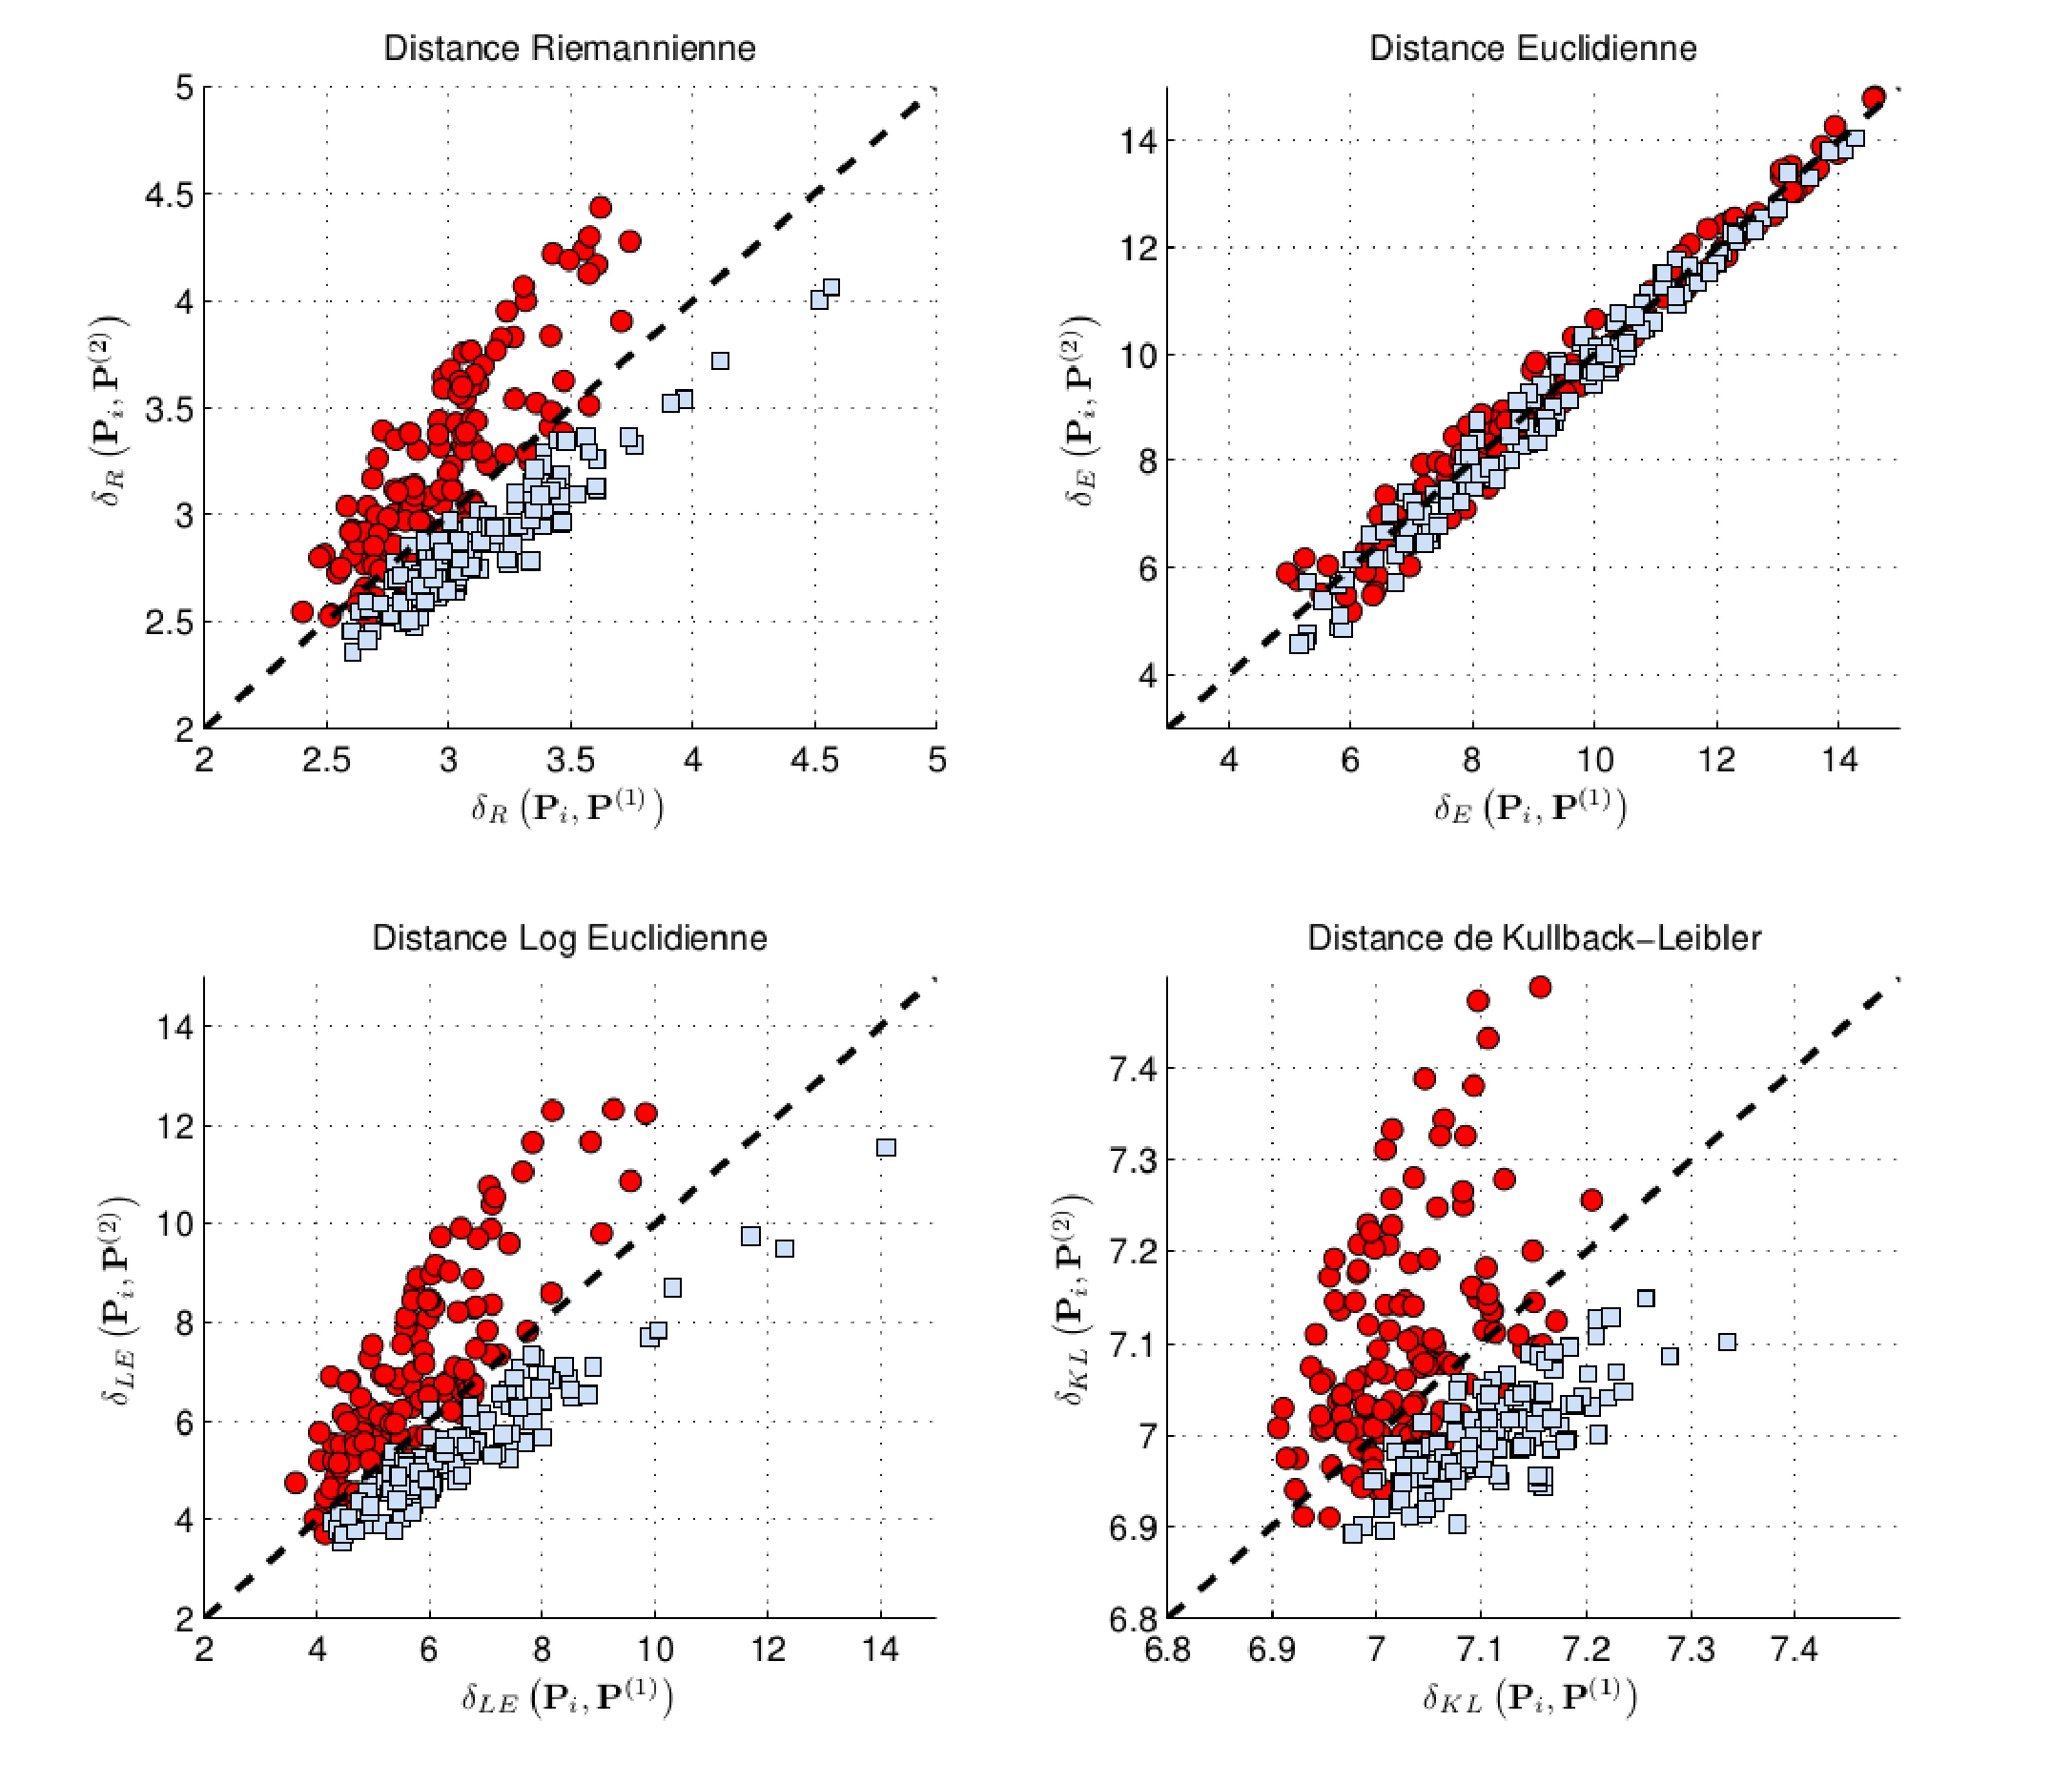
\includegraphics[width=.8\textwidth]{imgs/sep2.eps}
  \caption{\citep{BARACHANT2013172} Separation of covariance matrices of two classes. The x axis represents the Riemannian distance of each covariance matrix $\Sigma_i$ of class (1) to the mean covariance matrix $\Sigma^{(1)}$ of class 1. The y axis represents the Riemannian distance of each covariance matrix $\Sigma_i$ of class (2) to the mean covariance matrix $\Sigma^{(2)}$ of class 2.}
  \end{center}
\end{figure}

\begin{figure}[H]
\begin{center}
  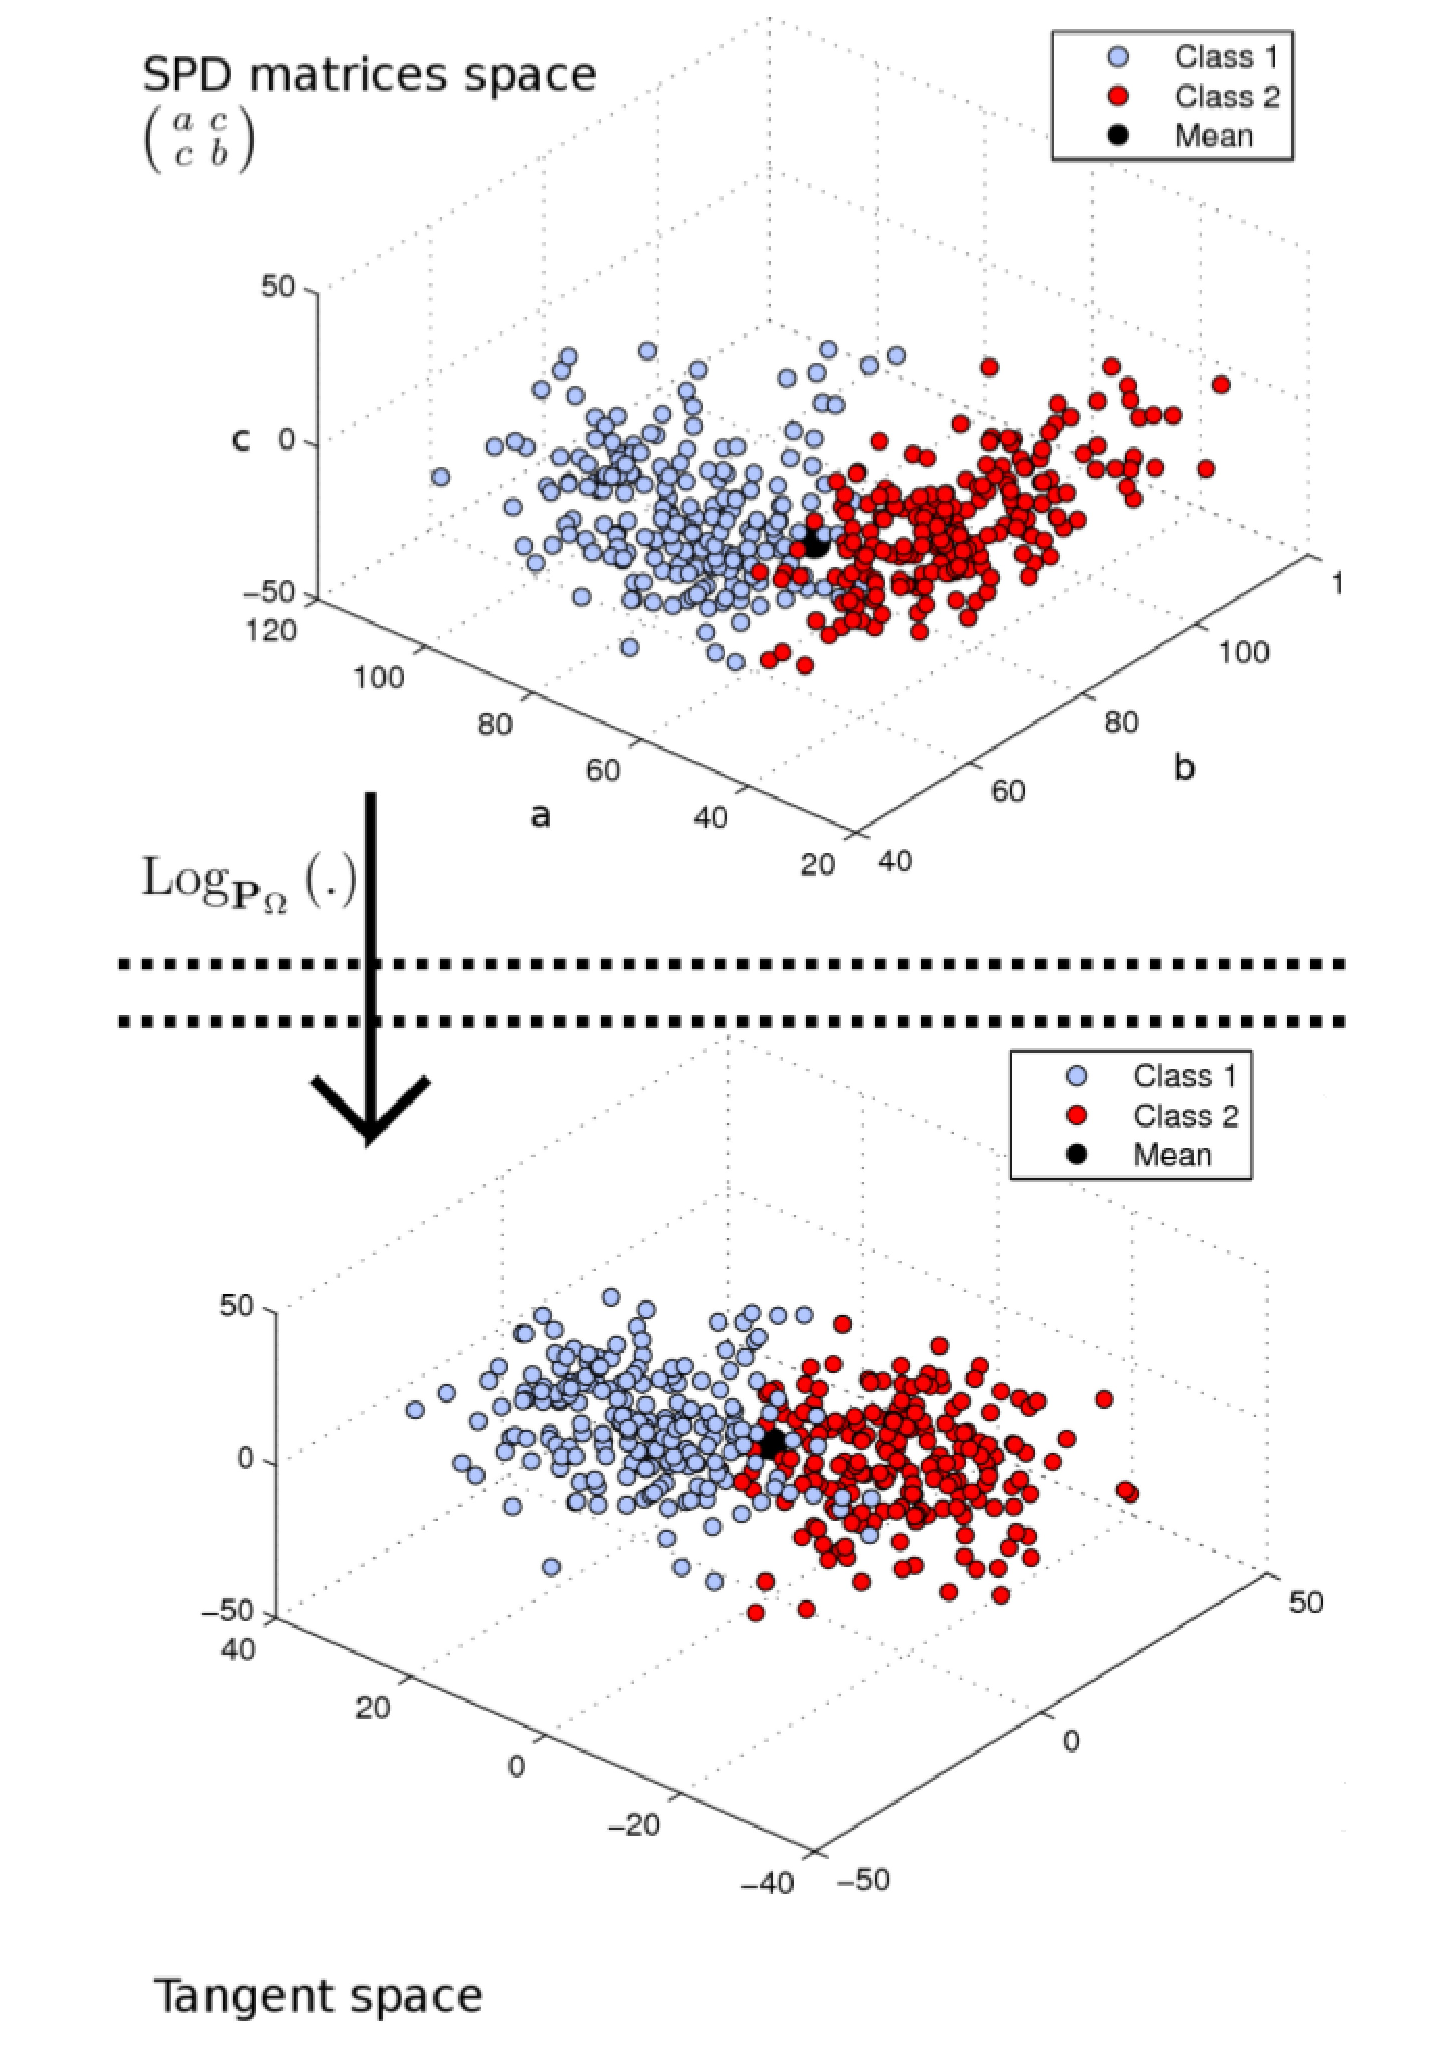
\includegraphics[width=.8\textwidth]{imgs/ts.eps}
  \caption{\citep{BARACHANT2013172} Example of a projection from the SPD matrices space to the corresponding tangent space}
  \end{center}
\end{figure}


\section{Comparison with other models}

Here is a summary of the four different models and approaches we considered:
\begin{itemize}
  \item A Support Vector Machine with Riemannian-based kernel taking the curvature of the manifold into account
  \item A naive approach based on low frequencies with a Random Forest
  \item A Logistic Regression learning from Power Spectral Densities
  \item A raw signal classification with a Convolutional Neural Network
\end{itemize}
For more details, please refer to our notebook:
\textit{Hand motions classification using non-invasive EEG recordings}.


\begin{figure}[!h]
\begin{center}
  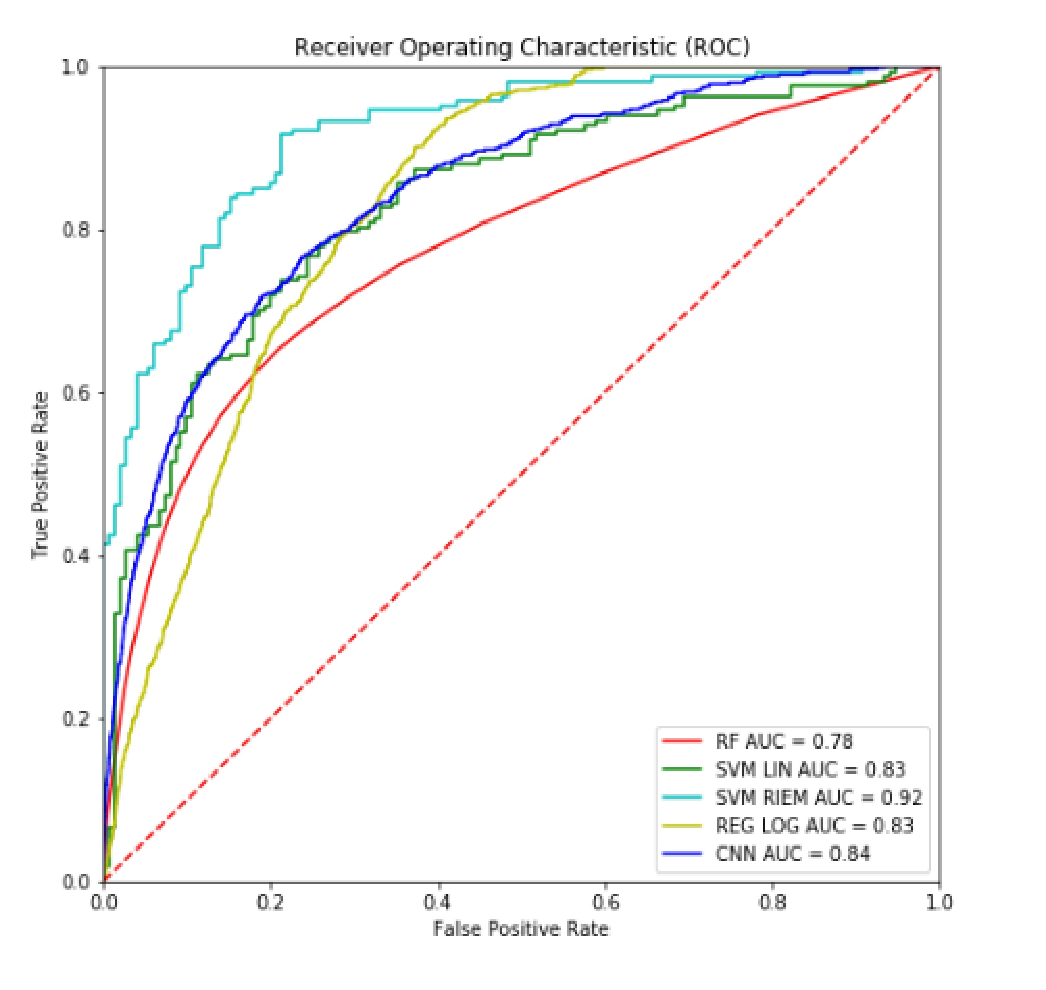
\includegraphics[width=.7\textwidth]{imgs/auc.eps}
  \end{center}
\end{figure}


\newpage

\bibliographystyle{apalike}
\bibliography{report}


\end{document}
